\documentclass{article}
\linespread{1.3}
\usepackage[margin=50pt]{geometry}
\usepackage{amsmath, amsthm, amssymb, amsthm, tikz, fancyhdr, graphicx, systeme}
\pagestyle{fancy}
\renewcommand{\headrulewidth}{0pt}
\newcommand{\changefont}{\fontsize{15}{15}\selectfont}

\fancypagestyle{firstpageheader}{
  \fancyhead[R]{
    \changefont
    \parbox[t]{4cm}{ % Adjust width as needed
      Michael Huang\\
      EN.625.603.84\\
      Problem Set \#4
    }
  }
}

\begin{document}

\thispagestyle{firstpageheader}
{\Large 

\section*{3.12.9.}
Calculate \(E(Y^3)\) for a random variable whose moment-generating function is \(M_Y(t) = e^{t^2/2}\).
\\
\\
By definition, we can find the expectation of \(Y^3\) given the moment-generating function  by taking the third derivative and evaluating at \(t=0\). Let's start differentiating:
\\
\[
M_Y'(t) = \frac{\partial}{\partial t} e^{t^2/2} = e^{t^2/2} \cdot \frac{2t}{2} = e^{t^2/2}t
\]
Then, use the product rule for the following:
\[
M_Y''(t) = \frac{\partial}{\partial t} e^{t^2/2}t = e^{t^2/2} \cdot \frac{2t}{2} \cdot t + e^{t^2/2} \cdot 1 = e^{t^2/2}t^2 + e^{t^2/2} = e^{t^2/2}(t^2 + 1)
\]
\[
M_Y'''(t) = \frac{\partial}{\partial t} (e^{t^2/2}(t^2 + 1)) = (e^{t^2/2} \cdot \frac{2t}{t} \cdot (t^2 + 1)) + (e^{t^2/2} \cdot 2t) 
\]
\[
= e^{t^2/2}(t^3 + t + 2t) = e^{t^2/2}(t^3 + 3t)
\]
\\ 
Now taking \(M_Y'''(0)\):
\[
M_Y'''(0) = e^{0^2/2}(0^3 + 3 \cdot 0) = 1(0) = \fbox{\(\mathbf{0}\)}
\]

\section*{3.12.16.}
Find the variance of \(Y\) if \(M_Y(t) = \frac{e^{2t}}{1 - t^2}\).
\\
\\
By definition, we know that the variance is \(Var(Y) = E(Y^2) - E(Y)^2\). Given the moment generating function, we can derive each of these terms as \(E(Y) = M_Y'(0)\) and \(E(Y^2) = M_Y''(0)\) respectively. Once again, let's start differentiating, first using the quotient rule:
\[
M_Y'(t) = \frac{\partial}{\partial t} \frac{e^{2t}}{1 - t^2} = \frac{e^{2t} \cdot 2 \cdot (1-t^2) - e^{2t} \cdot -2t}{(1-t^2)^2} = \frac{e^{2t} (2 -2t^2 + 2t)}{(1-t^2)^2}
\]
We can now determine that \(E(Y) = M_Y'(0) = \frac{e^{0} \cdot (2 - 0 + 0)}{(1-0)^2} = \frac{1 \cdot 2}{1} = 2 \). 
Let's continue differentiating using the quotient rule and product rule for the numerator:
\[
M_Y''(t) = \frac{\partial}{\partial t} \frac{e^{2t} \cdot (2 -2t^2 + 2t)}{((1-t^2)^2)^2} 
\]
\[
= \frac{[(2e^{2t}(2 - 2t^2 + 2t) + e^{2t}(-4t + 2))] \cdot (1-t^2)^2 - e^{2t} (2 - 2t^2 + 2t) \cdot 2 \cdot (1 - t^2) \cdot -2t}{(1-t^2)^4}
\]
\[
= \frac{[e^{2t}(4 - 4t^2 + 4t - 4t + 2)] \cdot (1-t^2)^2 - e^{2t}(2 - 2t^2 + 2t)(-4t + 4t^3) }{(1-t^2)^4}
\]
\[
= \frac{e^{2t}(6 - 4t^2)(1-t^2)^2 - e^{2t}(2 - 2t^2 + 2t)(-4t + 4t^3) }{(1-t^2)^4}
\]
We can now determine that 
\[
E(Y^2) = M_Y''(0) = \frac{e^{0}(6 - 0)(1 - 0)^2 - e^{0}(2 - 0 + 0)(0 + 0) }{(1 - 0)^4}
\]
\[
= \frac{6 - 0}{1} = 6
\]
Putting this all together, we can find the variance:
\[
Var(Y) = E(Y^2) - E(Y)^2 = 6 - 2^2 = 6 - 4 = \fbox{\(\mathbf{2}\)}
\]

\section*{4.2.7.}
According to an airline industry report, roughly one piece of luggage out of every two hundred that are checked is lost. Suppose that a frequent-flying businesswoman will be checking one hundred twenty bags over the course of the next year. Approximate the probability that she will lose two or more pieces of luggage.
\\
\\
We can approximate this using the Poisson distribution. We have \(p\) as \(\frac{1}{200}\), and \(n\) as 120 (bags). We can set up the probability as being \(1 - P(X \leq 1)\):
\[
P(X \geq 2) = 1 - P(X \leq 1)
\]
\[
= 1 - \sum_{k=0}^{1} \binom{120}{k} \frac{1}{200}^k (1-\frac{1}{200})^{120-k}
\]
\[
= 1 - \sum_{k=0}^{1} e^{-120 \cdot \frac{1}{200}} \frac{(-120 \cdot \frac{1}{200})^k}{k!}
\]
\[
= 1 - \sum_{k=0}^{1} e^{-0.6} \frac{0.6^k}{k!}
\]
\[
= 1 -  e^{-0.6}\frac{0.6^1}{1!} - e^{-0.6} \frac{0.6^0}{0!}
\]
\[
= 1 -  0.6e^{-0.6} - e^{-0.6}
\]
\[
\approx \fbox{\(\mathbf{0.12190138225}\)}
\]

\section*{4.2.26.}
Suppose that commercial airplane crashes in a certain country occur at the rate of 2.5 per year.

\subsection*{(a)} 
Is it reasonable to assume that such crashes are Poisson events? Explain.
\\
\\
It seems reasonable to assume that such crashes are Poisson events, since they seem to be countable and relatively independent events from each other with no interpendencies and occur at a somewhat constant rate per unit of time (year).

\subsection*{(b)} 
What is the probability that four or more crashes will occur next year?
\\
\\
We can calculate using the Possion distribution. We have \( \lambda = 2.5 \) crashes per year. We can therefore calculate as follows:
\[
P(X \geq 4) = 1 - P(X \leq 3) = 1 - \sum_{k=0}^{3} e^{-2.5} \frac{2.5^k}{k!} 
\]
\[
= 1 - e^{-2.5} \frac{2.5^3}{3!}  - e^{-2.5} \frac{2.5^2}{2!} - e^{-2.5} \frac{2.5^1}{1!} - e^{-2.5} \frac{2.5^0}{0!}
\]
\[
= 1 - e^{-2.5} (\frac{2.5^3}{6} + \frac{2.5^2}{2} + \frac{2.5}{1} + 1) 
\]
\[
= 1 - 0.08208499862 \cdot (\frac{225}{24})
\]
\[
= 1 - 0.76954686206
\]
\[
\approx \fbox{\(\mathbf{0.23045313794}\)}
\]

\subsection*{(c)} 
What is the probability that the next two crashes will occur within three months of one another?
\\
\\
We first can convert the ratio to months, so the monthly rate would be \( \lambda = \frac{2.5}{12} = \frac{5}{24}\). For a Poisson process, the time between events is exponentially distributed with rate \( \lambda \), so we can just take this simply as 
\[
P(T \leq 3) = 1 - e^{-\lambda \cdot 3} = 1 - e^{-\frac{5}{24} \cdot 3} = 1 - e^{-\frac{5}{8}} = 1 - 0.53526142851 \approx \fbox{\(\mathbf{0.46473857149}\)}
\]

\section*{4.3.2.}
Let Z be a standard normal random variable. Use Appendix Table A.1 to find the numerical value for each of the following probabilities. Show each of your answers as an area under \(f_Z(z)\).

\subsection*{(a)} 
\( P(0 \leq Z \leq 2.07) = .98077 - 0.5 = \fbox{\(\mathbf{0.48077}\)} \)
\\
\\
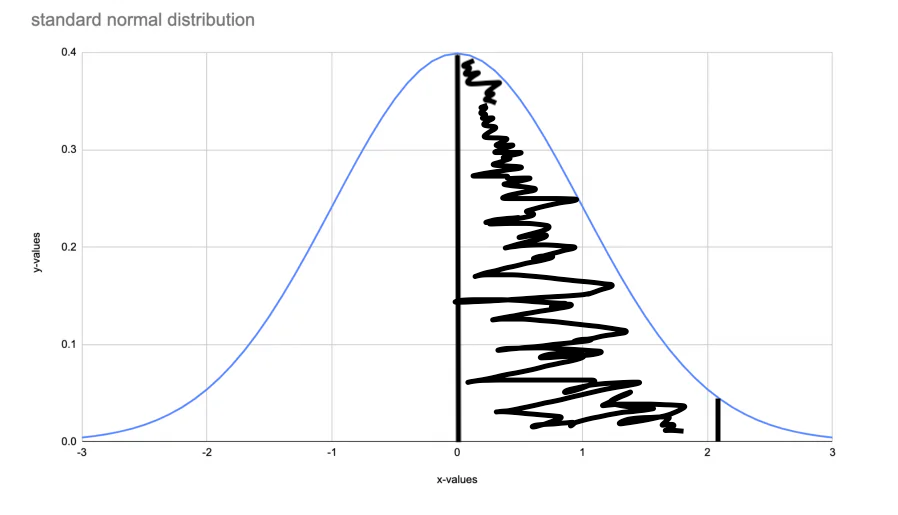
\includegraphics[width=500pt]{curve_2a.png}

\subsection*{(b)} 
\( P(-0.64 \leq Z < -0.11) = .45620 - .26109 = \fbox{\(\mathbf{0.19511}\)} \)
\\
\\
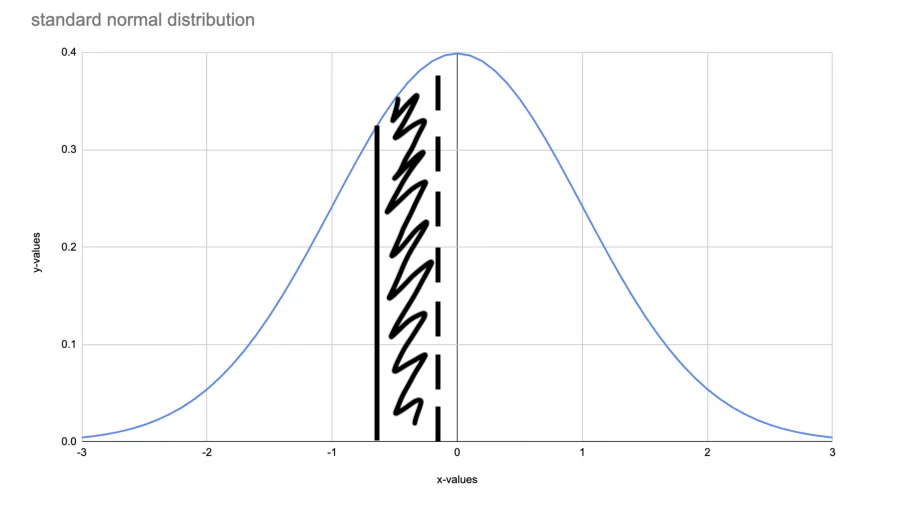
\includegraphics[width=500pt]{curve_2b.png}

\subsection*{(c)} 
\( P(Z > -1.06) = 1 - .14457 = \fbox{\(\mathbf{0.85543}\)} \)
\\
\\
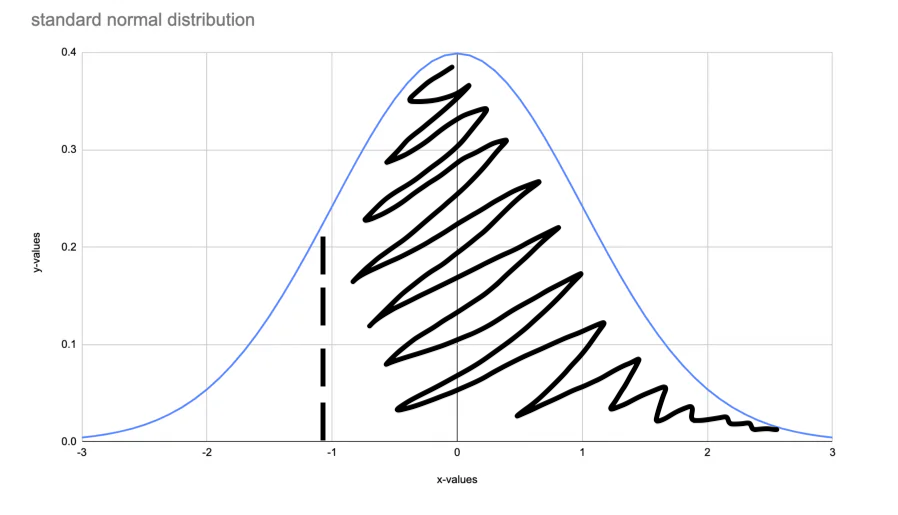
\includegraphics[width=500pt]{curve_2c.png}

\subsection*{(d)} 
\( P(Z < -2.33) = \fbox{\(\mathbf{0.00990}\)} \)
\\
\\
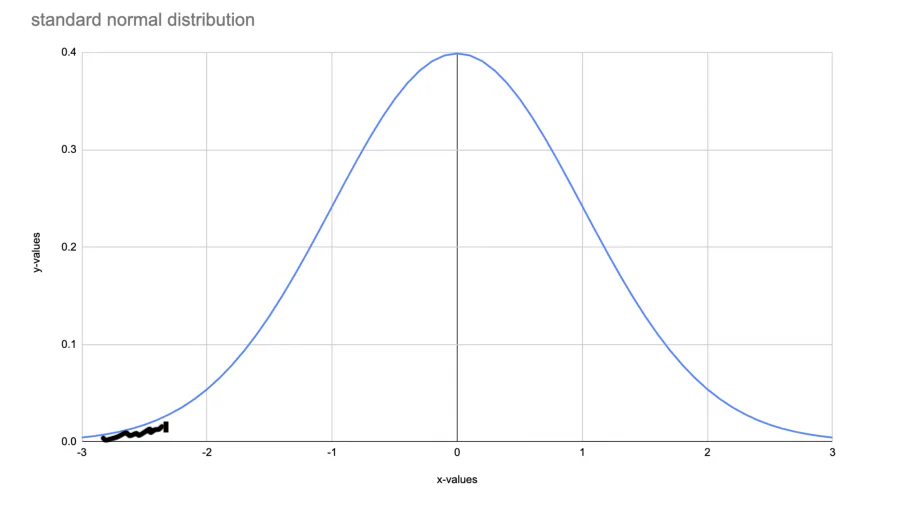
\includegraphics[width=500pt]{curve_2d.png}

\subsection*{(e)} 
\( P(Z \geq 4.61) = \fbox{\(\mathbf{0}\)} \) 
\\
\\
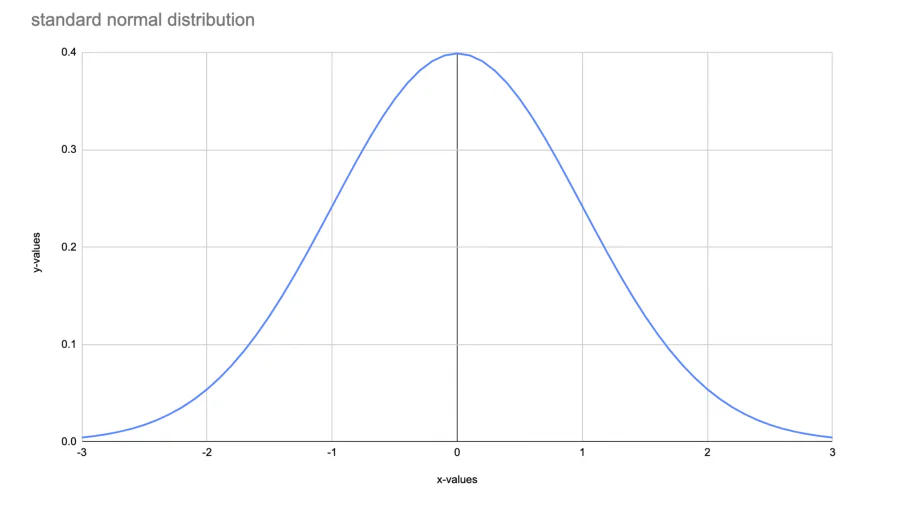
\includegraphics[width=500pt]{curve_2e.png}

\section*{4.3.5.}
Assume that the random variable \(Z\) is described by a standard normal curve \(f_Z(z)\). For what values of \(z\) are the following statements true?

\subsection*{(a)} 
\( P(Z \leq z) = 0.33 \)
\\
\\
Looking at the table, we look for where the value is about 0.33, i.e. where the area under the curve to the left is about 0.33. The value of \(z\) that fits the best is \(\fbox{\(\mathbf{-1.84}\)}\) with value 0.3288.

\subsection*{(b)} 
\( P(Z \geq z) = 0.2236 \)
\\
\\
Looking at the table, we look for where the value is about 1 - 0.2236 = 0.7764. The value of \(z\) that fits the best is \fbox{\(\mathbf{0.76}\)} with value 0.77637.

\subsection*{(c)} 
\( P(-1.00 \leq Z \leq z) = 0.5004 \)
\\
\\
Looking at the table, we look for where the value is about 0.15866 + 0.5004 = 0.65906, since we want to account for the area to the left of -1.00 as well. The value of \(z\) that fits the best is \fbox{\(\mathbf{0.41}\)} with value 0.65906.

\subsection*{(d)} 
\( P(-z < Z < z) = 0.80 \)
\\
\\
Looking at the table, we look for where the value is about \( (1 - 0.8) \div 2 = 0.1\). This is because we need the middle area covered under the curve to be symmetrical with 0.4 on either side, so we have 0.1 left on the left end area to look for. The value of \(z\) that fits the best is \fbox{\(\mathbf{2.33}\)} with value 0.00990 at -2.33, since the distribution is symmetric.

\subsection*{(e)} 
\( P(z \leq Z \leq 2.03) = 0.15 \)
\\
\\
Looking at the table, we look for where the value is about 0.97882 - 0.15 = 0.82882, since we want account for the area already covered to the left of 2.03. The value of \(z\) that fits the best is \fbox{\(\mathbf{0.95}\)} with value 0.82894.

\section*{4.3.9.}
Fifty-five percent of the registered voters in Sheridanville favor their incumbent mayor in her bid for re-election. If four hundred voters go to the polls, approximate the probability that

\subsection*{(a)} 
the race ends in a tie.
\\
\\
We can approximate the probability using the normal distribution. We have \(n = 400, p = 0.55\). Therefore, \(np = 400 \cdot 0.55 = 220\). To have a tie, we approximate \(P(X = 200) = P(199.5 < X < 200.5)\) with continuity correction, from which we can then standardize and find the probability using a standard normal distribution table like so: 
\[
P(199.5 < X < 200.5) = F_Z(\frac{200.5 - 400 \cdot 0.55}{\sqrt{400 \cdot 0.55 \cdot (1-0.55)}}) - F_Z(\frac{199.5 - 400 \cdot 0.55}{\sqrt{400 \cdot 0.55 \cdot (1-0.55)}})
\]
\[
= F_Z(\frac{-19.5}{\sqrt{99}}) - F_Z(\frac{-20.5}{\sqrt{99}}) = F_Z(-1.95982373976) - F_Z(-2.06032752128)
\]
\[
= F_Z(-1.96) - F_Z(2.06) = 0.02500 - 0.01970 = \fbox{\(\mathbf{0.0053}\)}
\]

\subsection*{(b)} 
the challenger scores an upset victory.
\\
\\
Using the same information as above, we also know that by definition, the challenger wins if \(P(X < 200) = P(X < 199.5)\), with continuity correction. We once again standardize and find the probability using a standard normal distribution table like so:
\[
P(X < 199.5) = F_Z(\frac{199.5 - 400 \cdot 0.55}{\sqrt{400 \cdot 0.55 \cdot (1 - 0.55)}}) = F_Z(-2.06032752128) 
\] 
\[
= F_Z(-2.06) = \fbox{\(\mathbf{0.01970}\)}
\]

% End of the large subsection
}

\end{document}